%%% template.tex
%%%
%%% This LaTeX source document can be used as the basis for your technical
%%% paper or abstract. Intentionally stripped of annotation, the parameters
%%% and commands should be adjusted for your particular paper - title, 
%%% author, article DOI, etc.
%%% The accompanying ``template.annotated.tex'' provides copious annotation
%%% for the commands and parameters found in the source document. (The code
%%% is identical in ``template.tex'' and ``template.annotated.tex.'')

\documentclass[conference]{acmsiggraph}

\TOGonlineid{45678}
\TOGvolume{0}
\TOGnumber{0}
\TOGarticleDOI{1111111.2222222}
\TOGprojectURL{}
\TOGvideoURL{}
\TOGdataURL{}
\TOGcodeURL{}

\title{CS 7616 - PS2 - Analysis of k-Nearest Neighbors}

\author{Daniel A. Castro Chin\thanks{e-mail:dcastro9@gatech.edu}\\Georgia Institute of Technology}
\pdfauthor{Daniel A. Castro Chin}

\keywords{nearest neighbor, knn, classification, pattern recognition}

\begin{document}

%% \teaser{
%%   \includegraphics[height=1.5in]{images/sampleteaser}
%%   \caption{Spring Training 2009, Peoria, AZ.}
%% }

\maketitle

\begin{abstract}

In this research endeavour we test the performance of k-Nearest Neighbors on three datasets, the Alcoholism Dataset, Bank-Note Authentication dataset, and the Diabetes in Pima Indians dataset, obtained from the UCI dataset repository \cite{Bache+Lichman:2013}. We split the datasets by randomly selecting 80 percent as training data, and the remaining as test data. We then take five random subsets for 20\%,50\%, and 80\% of the training data, and include the entire training dataset for a total of 16 training sets. We perform 2, 5, and leave one out cross validation for 10 values of k (odd numbers from 1 to 19) in order to obtain a robust analysis of our results. Lastly, we take the testing data and use our best methods to evaluate the remaining 20\%. We report these results for each of the datasets in the following three sections. We also perform normalization, weighting, and whitening of the data for the Alcoholism dataset, and whitening for the Bank-Note Authentication and Pima Indians dataset to observe changes in performance.

\end{abstract}

\begin{CRcatlist}
  \CRcat{I.3.3}{Computer Graphics}{Three-Dimensional Graphics and Realism}{Display Algorithms}
  \CRcat{I.3.7}{Computer Graphics}{Three-Dimensional Graphics and Realism}{Radiosity};
\end{CRcatlist}

\keywordlist

%% Use this only if you're preparing a technical paper to be published in the 
%% ACM 'Transactions on Graphics' journal.

\TOGlinkslist

%% Required for all content. 

\copyrightspace

\section{Introduction}

In this report we present the results of a specific classification technique on three datasets we obtain from the UCI Machine Learning repository. NOTE: We included supplemental figures at the end of the document which were not particularly interesting but were generated in the analysis. The remaining figures that are not pictured in this report can also be seen in the final results folder for each of the datasets.

\section{Alcoholism Dataset}
\subsection{Description}
The alcoholism dataset is represented by six attributes, and a binary classification on whether the patient has a liver disorder from excessive alcohol consumption. The alcoholism training dataset contained 302 data samples, and the testing set contained 45 samples to test on. It is important to note that distinctive to the other two datasets, we did not break down the initial data into training and testing as the set was already divided for us in the problem set description.
\subsection {Attempted Methods}
For the alcoholism dataset we performed a variety of preliminary tests in order to observe the effects it had on the data. We first parsed the original dataset into six different representations. The first four representations involved using the original dataset, normalizing the data, normalizing and weighing the more significant attributes and whitening the data. The other two methods utilized a more recent method of hashing attributes for dimensionality reduction known as the Winner-Take-All hashing algorithm\cite{yagnik2011power}. Despite implementing this method and a specific distance metric for hash comparison (Hamming distance) it did not seem to provide better results so I opted for utilizing the following four representations.
\subsection {Results}
\subsubsection{Original Dataset}
\begin{table}[h]
\caption{Original Dataset - Best Results with k-Value}
\centering
\begin{tabular}{c c c c}
\hline\hline
TS \% & 2-Fold & 5-Fold & N-Fold \\ [0.5ex]
%heading
\hline
20 & 60.7\% - k=1 & 60.7\% - k=19 & 63.7\% - k=3 \\
50 & 63.3\% - k=17 & 64.4\% - k=11 & 65.4\% - k=15 \\
80 & 66.9\% - k=3 & 71.8\% - k=5 & 71.6\% - k=7 \\
100 & 69.2\% - k=13 & 68.3\% - k=11 & 72.8\% - k=7 \\
\hline
\end{tabular}
\label{alc_o_res_table}
\end{table}

\begin{figure}[h]
  \centering
  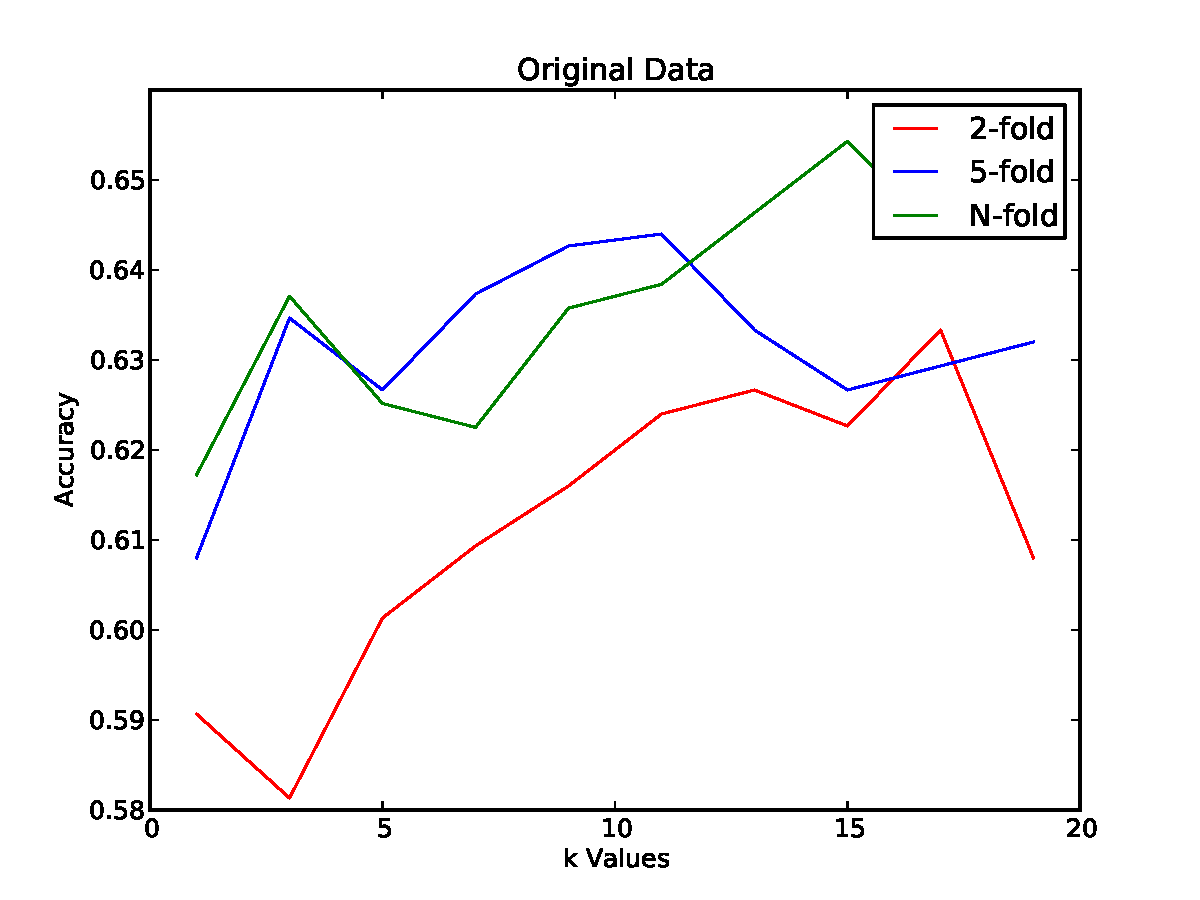
\includegraphics[width=2.8in]{images/alc_o_50.pdf}
  \caption{50\% of the TD. In this we see great stability and it is easier to view a trend based on the given k values.}
\end{figure}
\begin{figure}[h]
  \centering
  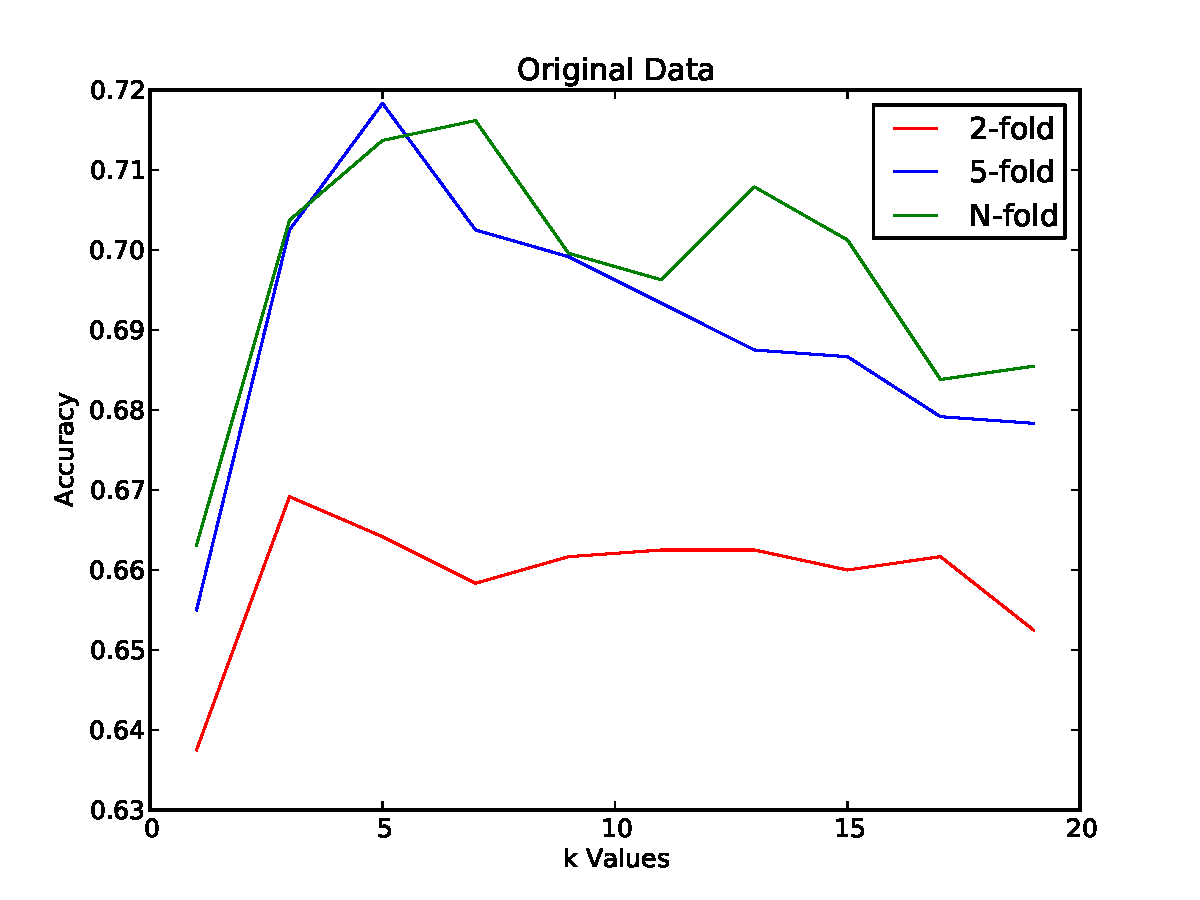
\includegraphics[width=2.8in]{images/alc_o_80.pdf}
  \caption{80\% of the TD. Here we see the greatest stability with 5-fold and N-fold CV converging to very similar classification results. 2-fold CV approaches a similar shape but at less accuracy.}
\end{figure}

The following are our best results for each of the types of cross validations, along with the value of k and type of cross validation that obtained the best accuracy. For conciseness, we only visualize the remaining results and include the actual data in our final\_results directory (see txt files). The best results were generally obtained by the N-Fold (Leave One Out) Cross Validation. 

Using 100\% of the training data expectedly obtained the best results, with a k of 7. Using 80\% of the data also obtained similar results, given the overlap in the data. The best result we obtain is 72.8\% using 100\% of the data and N-Fold Cross validation (this is expected because for every fold we are only leaving one sample out and using the remaining set for training). The analysis for each of the graphs is provided in their caption given that this assignment produced a large number of graphics.

This approach still outperformed the other three methods which we attempted, with whitening coming in as a close second. When we ran our best k against the testing sample, we obtained incredibly poor results. A number of the classifications were worse than chance (in which case we could have simply flipped the classification for a better than chance classification). The best performance was obtained at 80\% with 2-fold cross validation of the data and k=5, in which the testing data classified 62\% of the data correctly.

\subsubsection{Normalized Dataset}
In this case we normalize the data from 0 to 1 by obtaining the minimum and maximum of each attribute and scaling it. We scale all the parameters equally in this case in order to see the effect on performance. The best result we obtain is an accuracy of 66.6\% with k=7 for 50\% of the data using N-fold cross validation.
\begin{table}[h]
\caption{Normalized Dataset - Best Results with k-Value}
\centering
\begin{tabular}{c c c c}
\hline\hline
TS \% & 2-Fold & 5-Fold & N-Fold \\ [0.5ex]
%heading
\hline
20 & 59.0\% - k=19 & 63.0\% - k=11 & 64.7\% - k=19 \\
50 & 61.3\% - k=9 & 65.1\% - k=7 & 66.6\% - k=7 \\
80 & 62.9\% - k=9 & 63.1\% - k=19 & 65.6\% - k=9 \\
100 & 65.2\% - k=13 & 64.0\% - k=9 & 65.6\% - k=19 \\
\hline
\end{tabular}
\label{alc_n_res_table}
\end{table}

\begin{figure}[h]
  \centering
  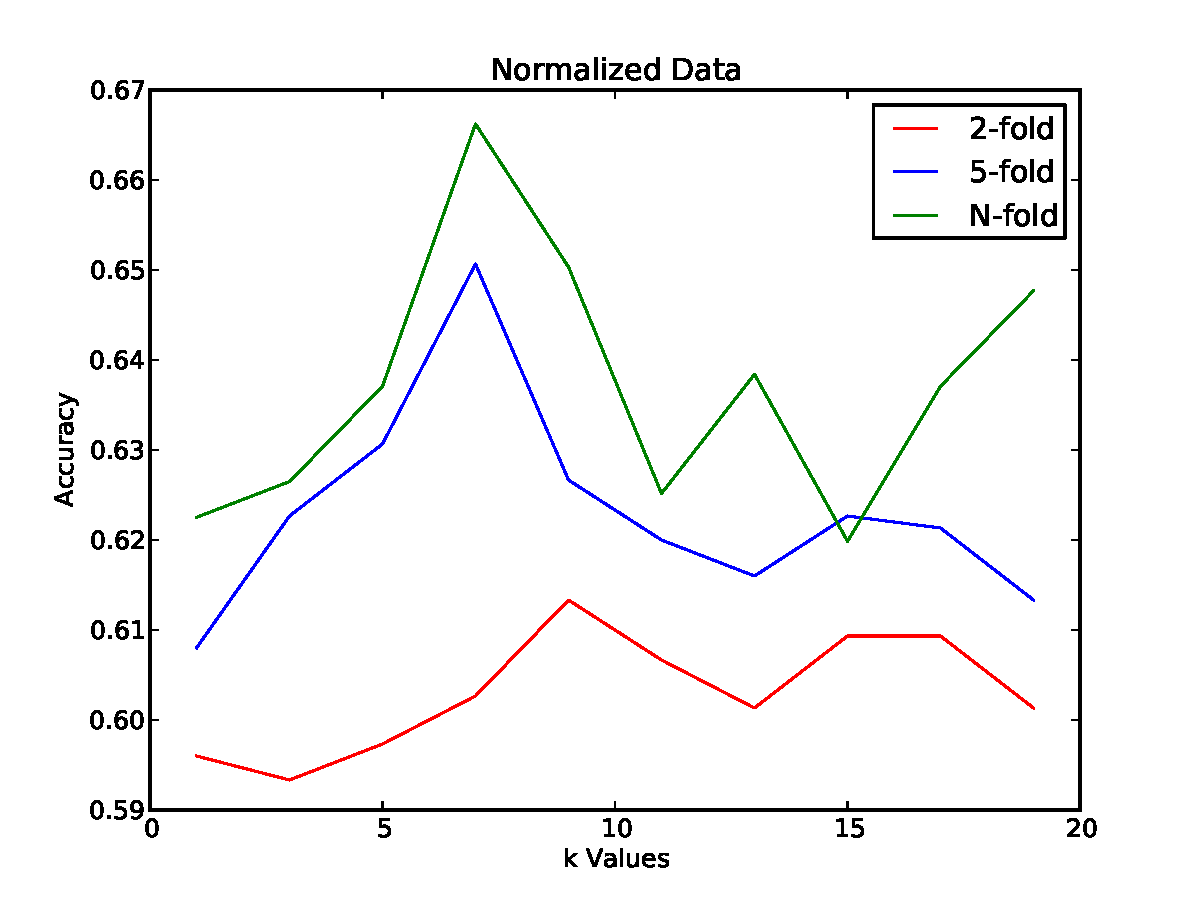
\includegraphics[width=2.8in]{images/alc_n_50.pdf}
  \caption{50\% of the TD. We see an interesting peak at approximately 7 neighbors, with a performance of 66.6\% for N-Fold validation.}
\end{figure}


\subsubsection{Normalized \& Weighted Dataset}
\begin{table}[h]
\caption{Normalized \& Weighted Dataset - Best Results with k-Value}
\centering
\begin{tabular}{c c c c}
\hline\hline
TS \% & 2-Fold & 5-Fold & N-Fold \\ [0.5ex]
%heading
\hline
20 & 61.6\% - k=15 & 60.7\% - k=7 & 62.0\% - k=9 \\
50 & 60.4\% - k=9 & 60.8\% - k=5 & 61.7\% - k=13 \\
80 & 61.5\% - k=17 & 63.3\% - k=13 & 63.5\% - k=1 \\
100 & 64.9\% - k=15 & 63.0\% - k=13 & 64.2\% - k=13 \\
\hline
\end{tabular}
\label{alc_nw_res_table}
\end{table}

Overall, the best result we obtain is 64.9\% using 100\% of the data, and a k=15. In this case we used arbitrary weights until we obtained a reasonable result based on intuition, but in future obtaining the eigen values of each attribute and performing some type of rank correlation metric as discussed previously with WTA hash may yield better results.

\begin{figure}[h]
  \centering
  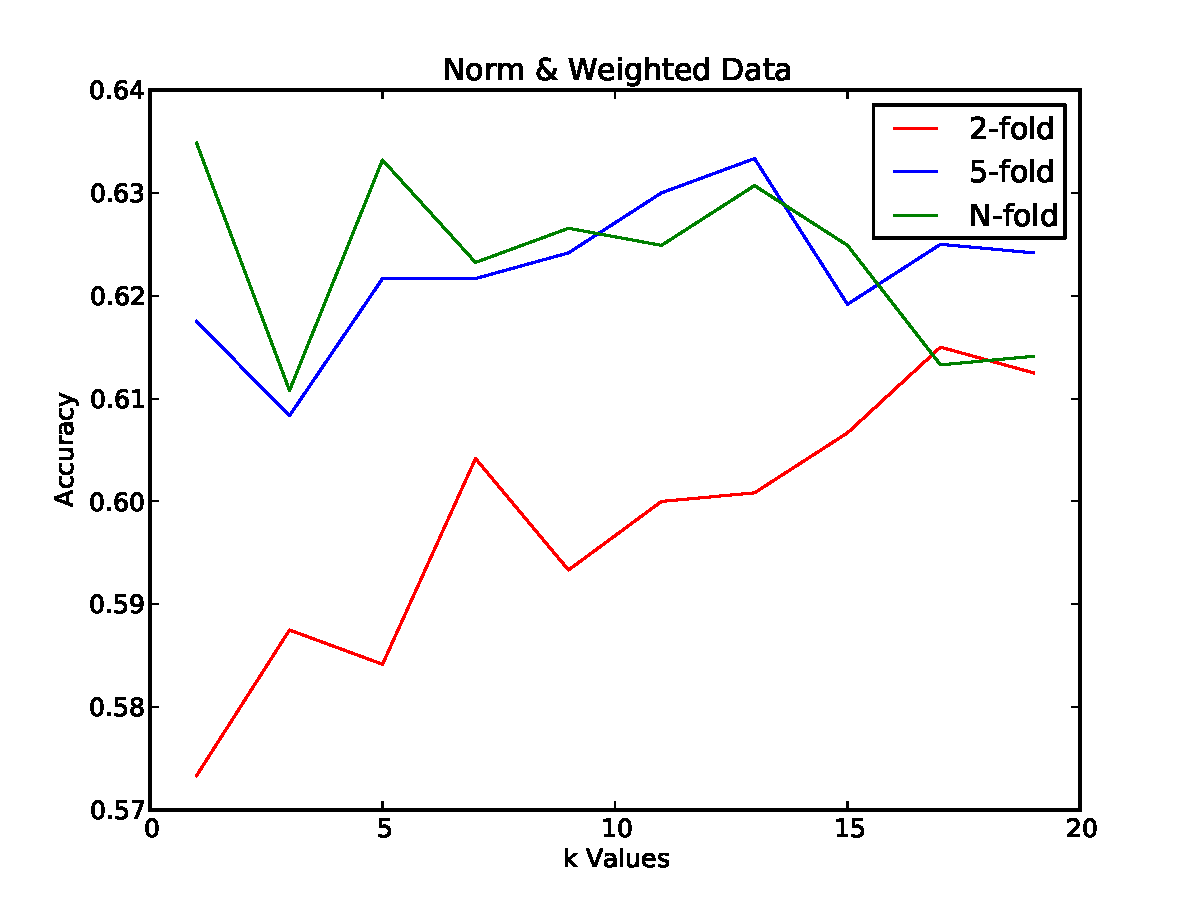
\includegraphics[width=2.8in]{images/alc_nw_80.pdf}
  \caption{80\% of the TD. It is interesting to see that 5-fold and N-fold cross validation follow a similar trend, while 2-fold cross validation approaches their results as k becomes larger.}
\end{figure}

\subsubsection{Whitened Dataset}
Whitening the data obtained much better results than simply normalizing or normalizing and weighing our attributes so we selected those approaches in the following two datasets. We did not see improvements over the original dataset but obtained better results than normalization and weighing certain attributes, at 70.2\% using 100\% of the TD with k=15.
\begin{table}[h]
\caption{Whitened Dataset - Best Results with k-Value}
\centering
\begin{tabular}{c c c c}
\hline\hline
TS \% & 2-Fold & 5-Fold & N-Fold \\ [0.5ex]
%heading
\hline
20 & 65.0\% - k=3 & 67.3\% - k=1 & 69.7\% - k=5 \\
50 & 63.3\% - k=13 & 66.8\% - k=15 & 64.9\% - k=17 \\
80 & 66.5\% - k=5 & 68.3\% - k=17 & 68.1\% - k=7 \\
100 & 71.2\% - k=7 & 69.3\% - k=5 & 70.2\% - k=15 \\
\hline
\end{tabular}
\label{alc_w_res_table}
\end{table}

\section{Bank-Note Authentication Dataset}
\subsection{Description}
The bank-note authentication dataset is represented by four attributes, and a binary classification on whether the data point is authentic or not. There are a total of 1372 data points in this dataset.
\subsection {Attempted Methods}
For this dataset we attempted to classify the data using the original data values, and whitened data values, as these were the best two methods that we learned from previous experiments. This is not necessarily a robust approach as each dataset can be distinctive in which methods of pre-processing work, but it was wise to only perform the best two as the sample space made this very computationally expensive. We obtained incredibly accurate results, approximating 100\% as we used the entire training sample, and even succeeded at the accuracy once we tested it on the testing data. 
\subsection {Results}
When compared to the testing data, seven out of the 12 methods (three CV methods for each of 20, 50, 80, and 100\% of the TD) obtained 100\% accuracy, most of which used a k=1 or k=3, with two using k=7. The whitened data did not perform as well, not obtaining 100\% accuracy for any of its tests against the testing data, but achieving 99.6\% accuracy on average.
\subsubsection{Original Dataset}
\begin{table}[h]
\caption{Original Dataset - Best Results with k-Value}
\centering
\begin{tabular}{c c c c}
\hline\hline
TS \% & 2-Fold & 5-Fold & N-Fold \\ [0.5ex]
%heading
\hline
20 & 98.6\% - k=1 & 99.6\% - k=1 & 99.7\% - k=1 \\
50 & 99.6\% - k=1 & 99.8\% - k=1 & 99.9\% - k=1 \\
80 & 99.8\% - k=1 & 99.9\% - k=1 & 68.1\% - k=1 \\
100 & 100.0\% - k=3 & 99.9\% - k=1 & 100.0\% - k=7 \\
\hline
\end{tabular}
\label{dba_n_res_table}
\end{table}
\subsubsection{Whitened Dataset}
For the whitened dataset we see how important the value of k is for this dataset. It decreases very directly when you use larger values of k, meaning that one neighbor is often the best classification. For reference see Figure \ref{fig:dbaw}.
\begin{table}[h]
\caption{Whitened Dataset - Best Results with k-Value}
\centering
\begin{tabular}{c c c c}
\hline\hline
TS \% & 2-Fold & 5-Fold & N-Fold \\ [0.5ex]
%heading
\hline
20 & 98.4\% - k=1 & 98.9\% - k=1 & 99.4\% - k=1 \\
50 & 99.6\% - k=1 & 99.8\% - k=1 & 99.9\% - k=1 \\
80 & 99.9\% - k=1 & 99.9\% - k=1 & 99.9\% - k=1 \\
100 & 99.7\% - k=1 & 99.9\% - k=1 & 100.0\% - k=1 \\
\hline
\end{tabular}
\label{dba_w_res_table}
\end{table}

\begin{figure}[h]
  \centering
  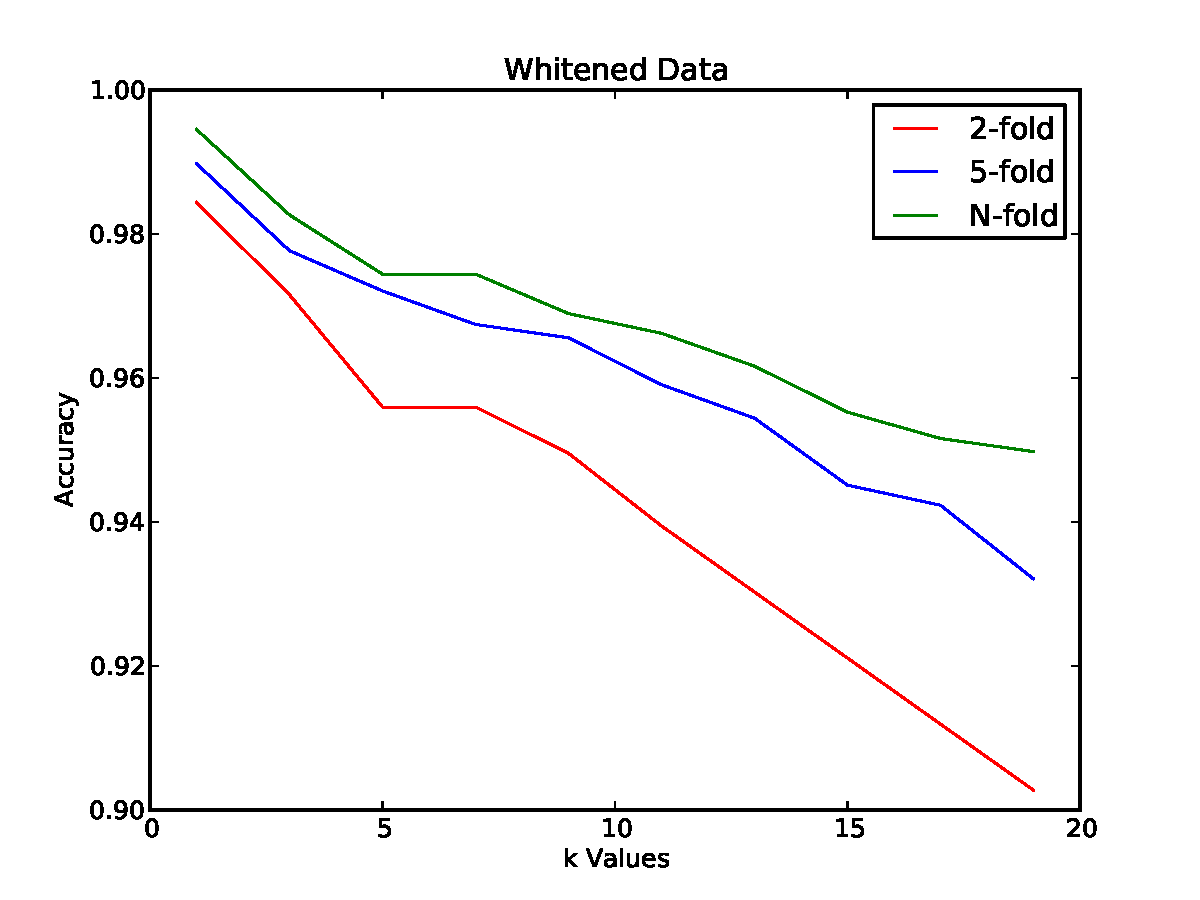
\includegraphics[width=2.8in]{images/dba_w_20.pdf}
  \caption{80\% of the TD. The dataset is fairly accurate with one neighbor regardless of the Cross Validation technique implemented.}
  \label{fig:dbaw}
\end{figure}

\section{Diabetes in Pima Indians Dataset}
\subsection{Description}
The Diabetes in Pima Indians dataset contained a total of 8 attributes and 768 instances. It was also a binary classification problem.
\subsection {Attempted Methods}
As with the previous dataset, we tried to classify the data using the original data values, and whitened data values and obtained decent results. 
\subsection {Results}
The original dataset obtained incredibly similar accuracies (low variance) when compared to the CV results. The accuracies varied from 69.4\% to 75.9\% accuracy, which is well within the range of the results that we saw when performing cross validation on all of our results for all k. The best accuracy was obtained with 50\% of the training data, for the accuracy of 75.9\%. The stability of the data can be reinforced by looking at Figure \ref{fig:pio} for the original data which depicts a correlation between all of the cross validation methods. It is important to note that this stability was seen at 80\% but the results at every percentage of data we took displayed a similar trend which means the data was consistent in its classification. This means we could have used less data points to achieve a similar accuracy.
\subsubsection{Original Dataset}
\begin{table}[h]
\caption{Original Dataset - Best Results with k-Value}
\centering
\begin{tabular}{c c c c}
\hline\hline
TS \% & 2-Fold & 5-Fold & N-Fold \\ [0.5ex]
%heading
\hline
20 & 72.6\% - k=7 & 72.0\% - k=9 & 72.9\% - k=7 \\
50 & 70.5\% - k=3 & 73.0\% - k=5 & 74.2\% - k=9 \\
80 & 72.4\% - k=5 & 73.4\% - k=11 & 73.8\% - k=13 \\
100 & 72.1\% - k=11 & 75.4\% - k=15 & 76.2\% - k=19 \\
\hline
\end{tabular}
\label{dba_n_res_table}
\end{table}

\begin{figure}[h]
  \centering
  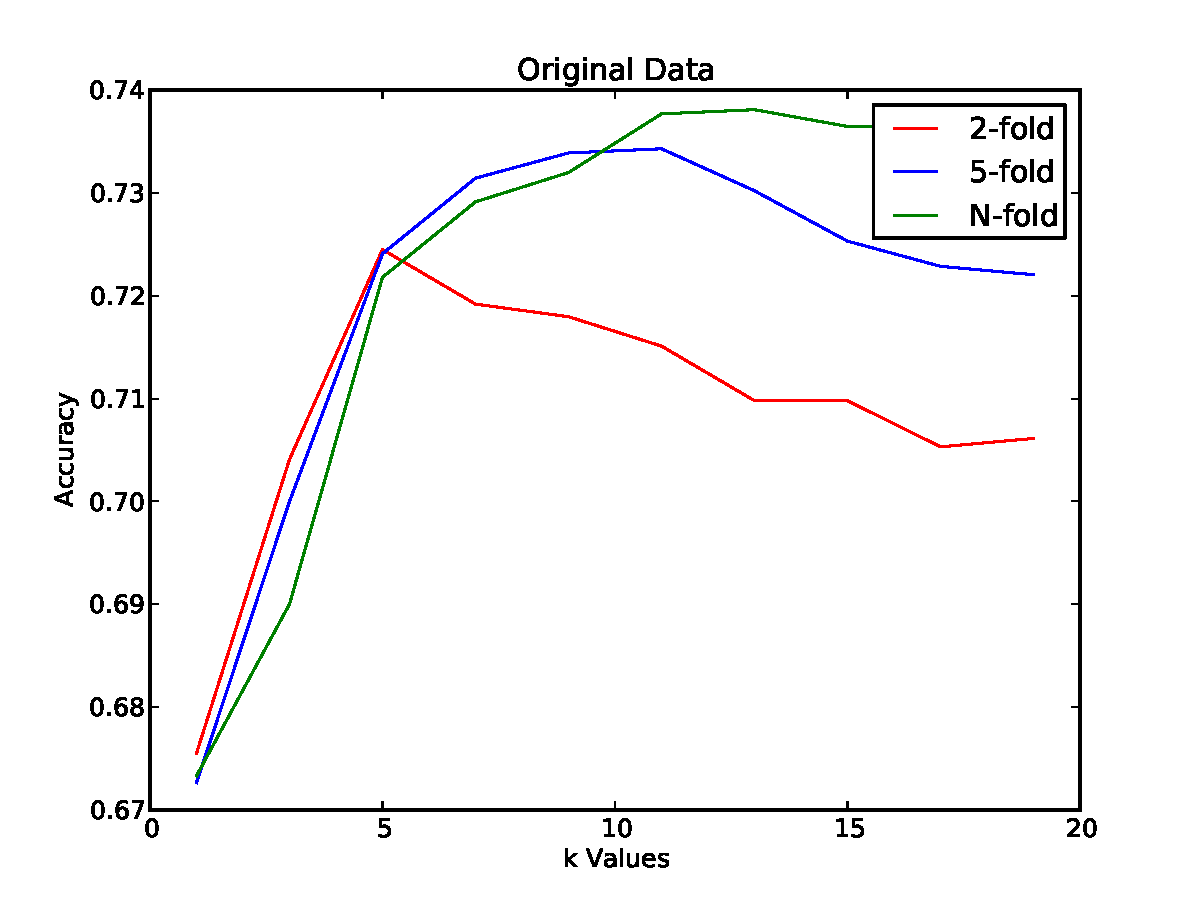
\includegraphics[width=2.8in]{images/pi_o_80.pdf}
  \caption{80\% of the TD. Here we can see how the cross validation results reach a peak at approximately k=10 and stop increasing in accuracy as k is increased. For 2-fold validation, the increase is seen a bit earlier.}
  \label{fig:pio}
\end{figure}

\subsubsection{Whitened Dataset}

\begin{table}[ht]
\caption{Whitened Dataset - Best Results with k-Value}
\centering
\begin{tabular}{c c c c}
\hline\hline
TS \% & 2-Fold & 5-Fold & N-Fold \\ [0.5ex]
%heading
\hline
20 & 61.9\% - k=13 & 61.8\% - k=19 & 63.1\% - k=9 \\
50 & 66.9\% - k=7 & 66.9\% - k=5 & 67.3\% - k=9 \\
80 & 69.9\% - k=7 & 70.7\% - k=13 & 71.2\% - k=17 \\
100 & 70.5\% - k=13 & 69.5\% - k=13 & 70.8\% - k=3 \\
\hline
\end{tabular}
\label{dba_w_res_table}
\end{table}

\begin{figure}[ht]
  \centering
  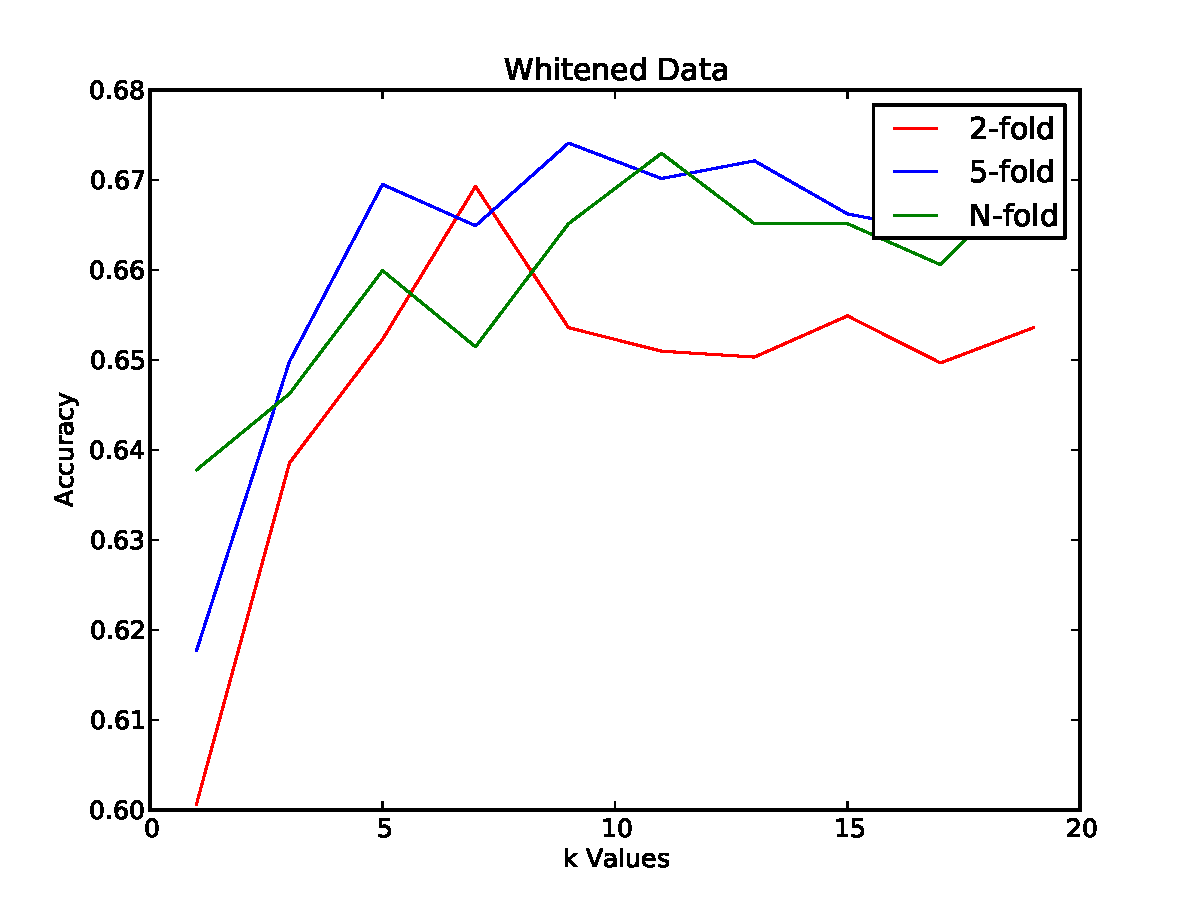
\includegraphics[width=2.8in]{images/pi_w_50.pdf}
  \caption{80\% of the TD. We see a similar trend here as we see in Figure \ref{fig:pio}, demonstrating the negligible effect of whitening in this scenario. }
  \label{fig:piw}
\end{figure}

Accuracy with the test data for the whitened dataset varied between 65.5\% and 72.1\% once again showing some variance but not as drastic as the variance we observed in the Alcoholics dataset. We include a figure of the whitened data for all cross validation attempts at 50\% of the training data in order to demonstrate the similarities it had with the original dataset (See Figure \ref{fig:piw}. This shows that whitening did not have a significant benefit in the classification.



\section{Conclusion}

Overall, the accuracy of k-Nearest Neighbors depended heavily on the dataset in which we tested. It was not robust to a change in attributes, and the choice of k was essential in obtaining better performance.

\section*{Acknowledgements}

This work was done for a course in Pattern Recognition taught by Professor Aaron Bobick at the College of Computing, at the Georgia Institute of Technology.

\bibliographystyle{acmsiggraph}
\bibliography{template}

\clearpage

\section{Remaining Figures}

Remaining figures are attached.

\begin{figure}[h]
  \centering
  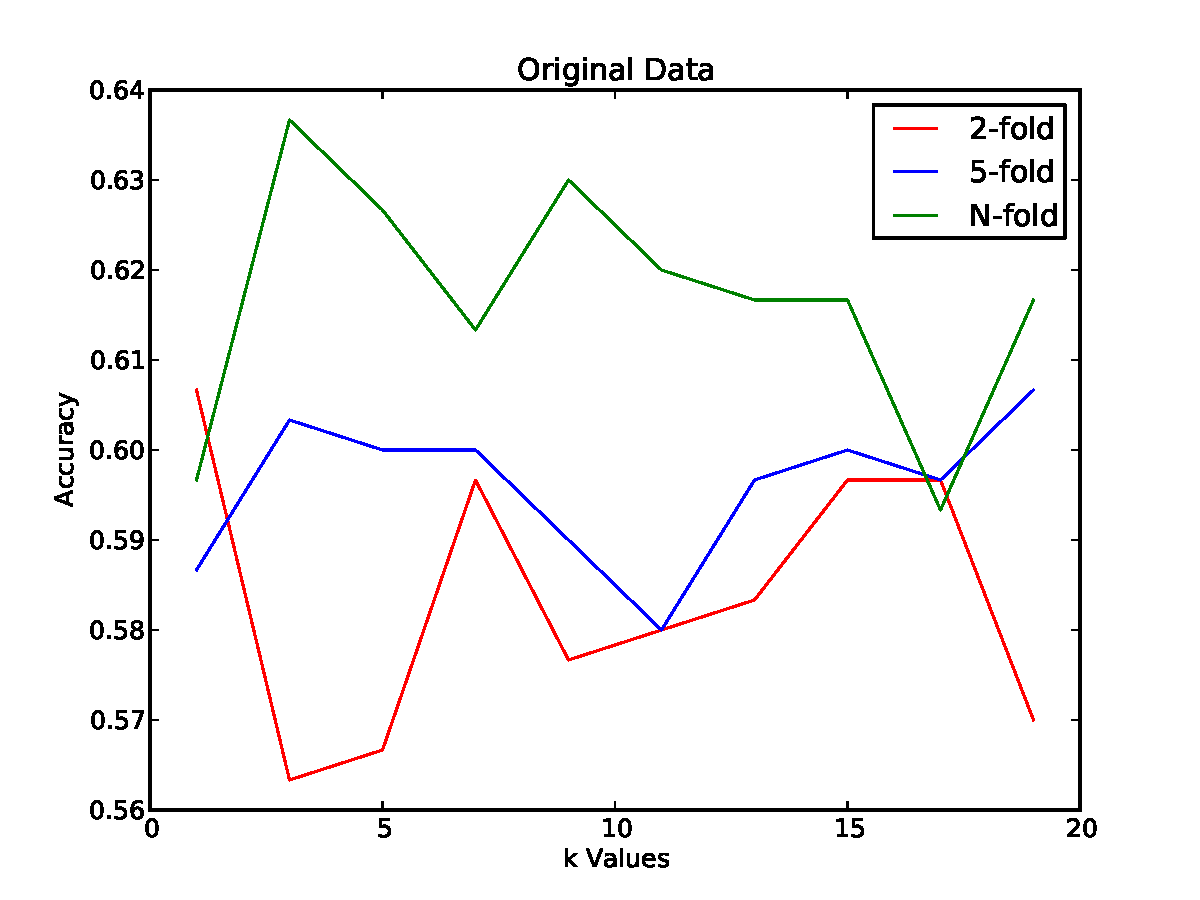
\includegraphics[width=2.8in]{images/alc_o_20.pdf}
  \caption{20\% of the TD. We see little to no correlation in the data here, which is expected given that you are randomly selecting 20 percent of the data, these training sets were unstable.}
\end{figure}

\begin{figure}[h]
  \centering
  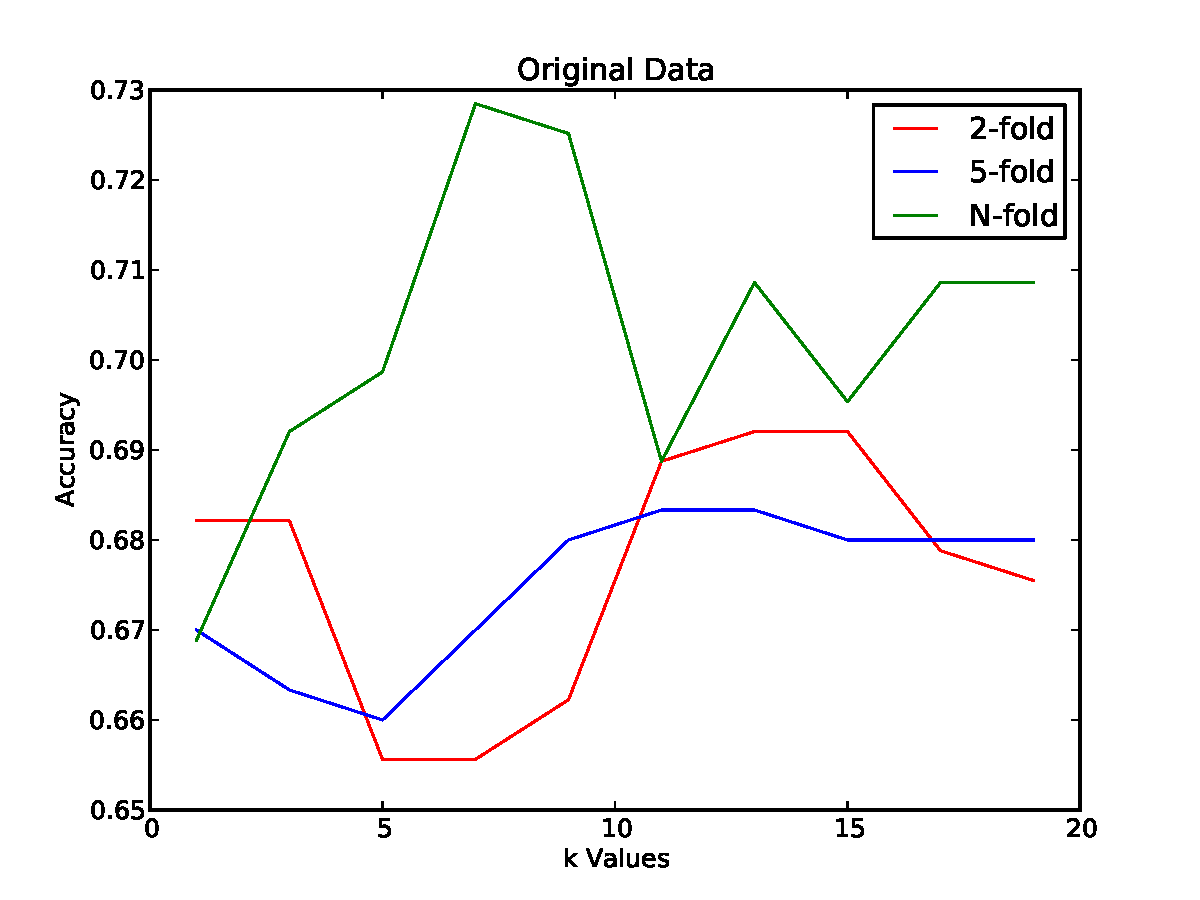
\includegraphics[width=2.8in]{images/alc_o_100.pdf}
  \caption{100\% of the TD. This becomes a lot more volatile because we are not running five iterations of a random subset (since this subset spans the entire set). Albeit the volatility, this achieves the highest accuracy with 7 nearest neighbors.}
\end{figure}

\begin{figure}[h]
  \centering
  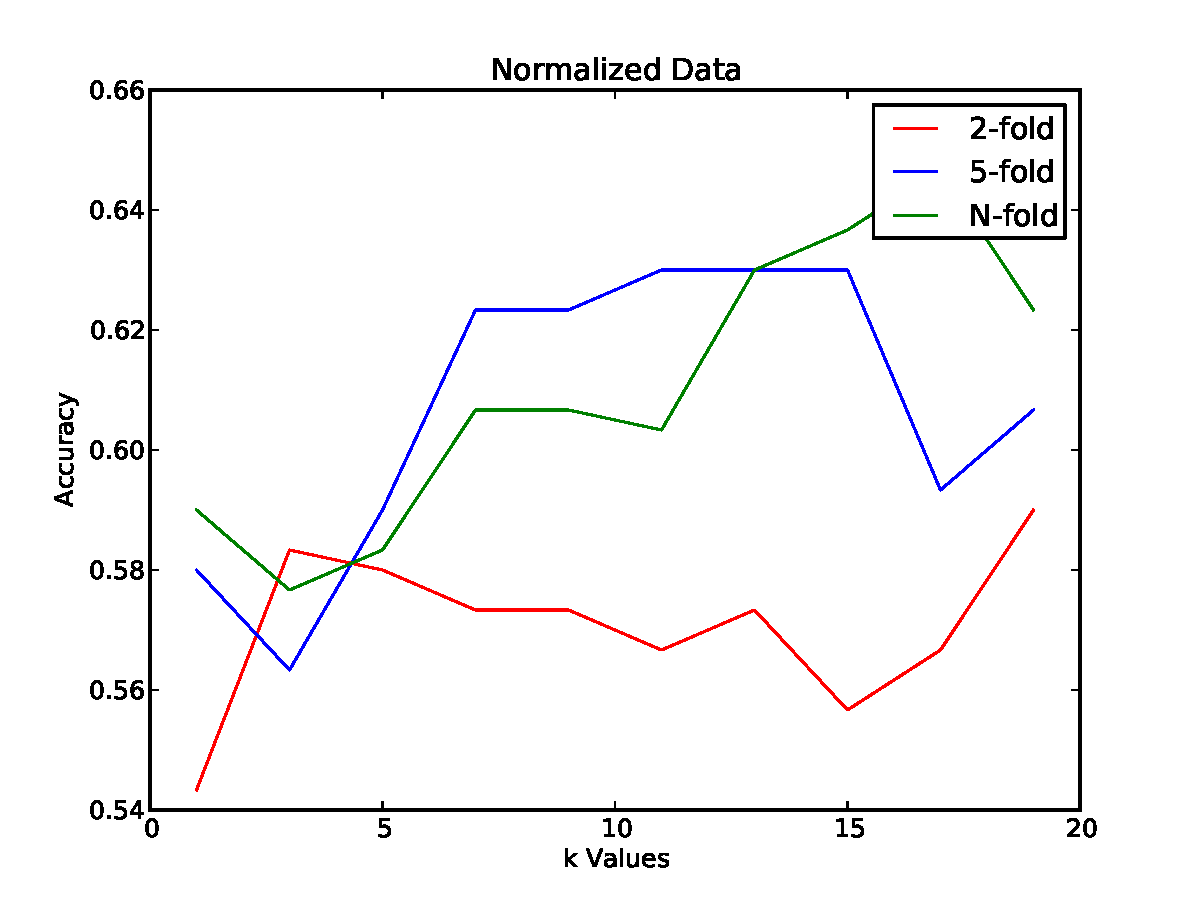
\includegraphics[width=2.8in]{images/alc_n_20.pdf}
  \caption{20\% of the TD. We see a slight increase up until approximately 15 nearest neighbors, but its hard to spot a trend. N-Fold validation outperforms the other CV methods at 19 nearest neighbors.}
\end{figure}

\begin{figure}[h]
  \centering
  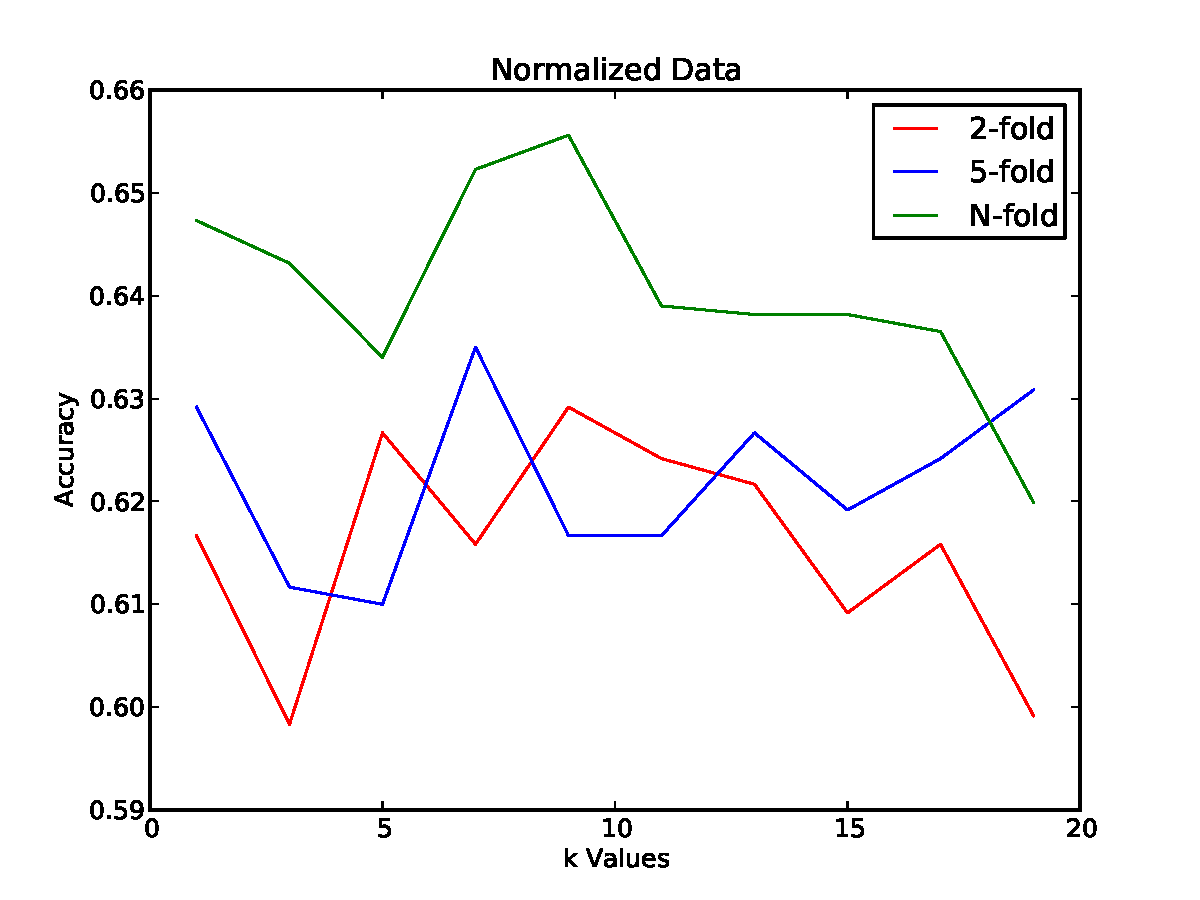
\includegraphics[width=2.8in]{images/alc_n_80.pdf}
  \caption{80\% of the TD. It is difficult to discern a trend in this visualization which we attribute to the granularity of the axes, the spikes are potentially due to noise in obtaining a random 80\% subset of the training data.}
\end{figure}

\begin{figure}[h]
  \centering
  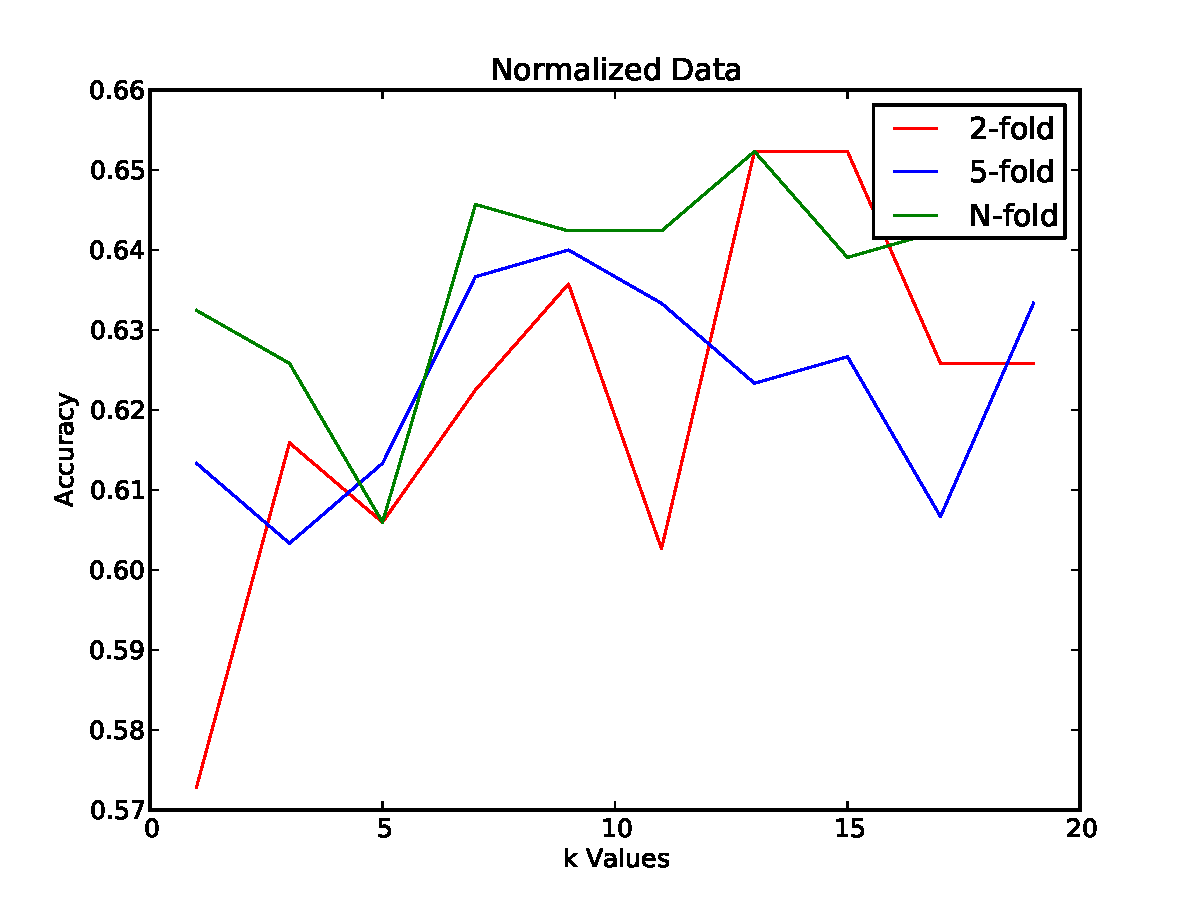
\includegraphics[width=2.8in]{images/alc_n_100.pdf}
  \caption{100\% of the TD. Here we see a trend with all methods of cross validation, although there is a significant amount of noise between 61 and 65\% accuracy that is hard to attribute to a change in k.}
\end{figure}

\begin{figure}[h]
  \centering
  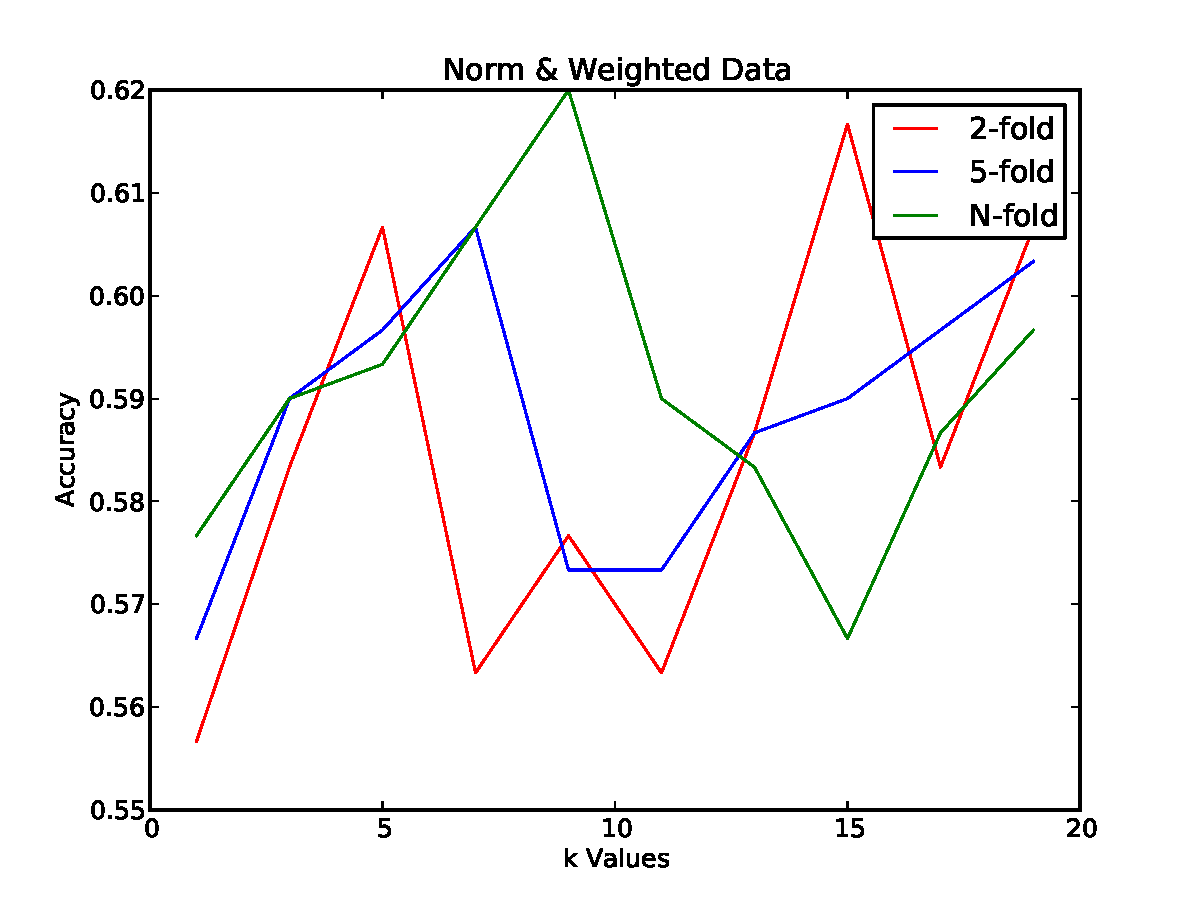
\includegraphics[width=2.8in]{images/alc_nw_20.pdf}
  \caption{20\% of the TD. We see the data follow a similar trend and reach a peak around 5-10 k values, and then dropping down, with 2-fold having the largest instability.}
\end{figure}

\begin{figure}[h]
  \centering
  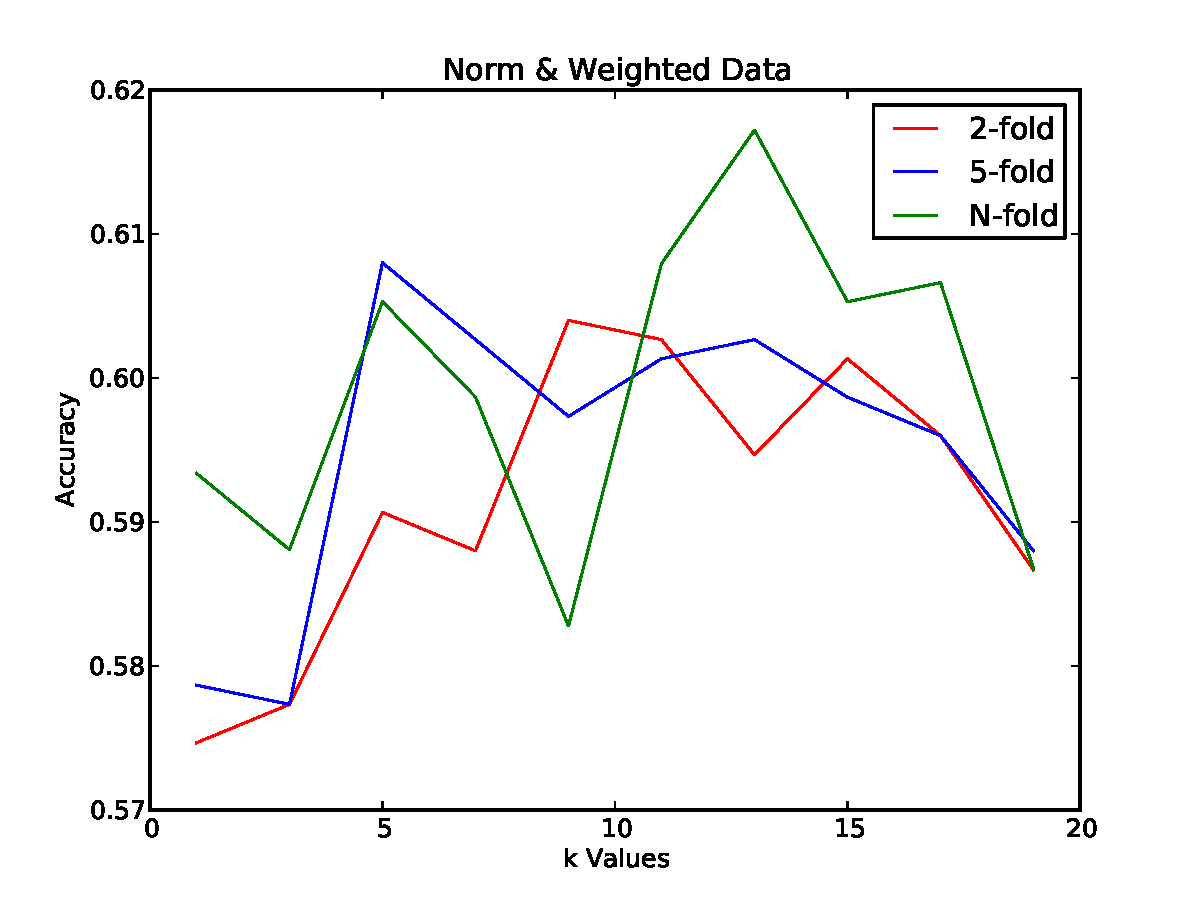
\includegraphics[width=2.8in]{images/alc_nw_50.pdf}
  \caption{50\% of the TD. Here the cross validation methods follow a similar trend, increase towards k=13.}
\end{figure}

\begin{figure}[h]
  \centering
  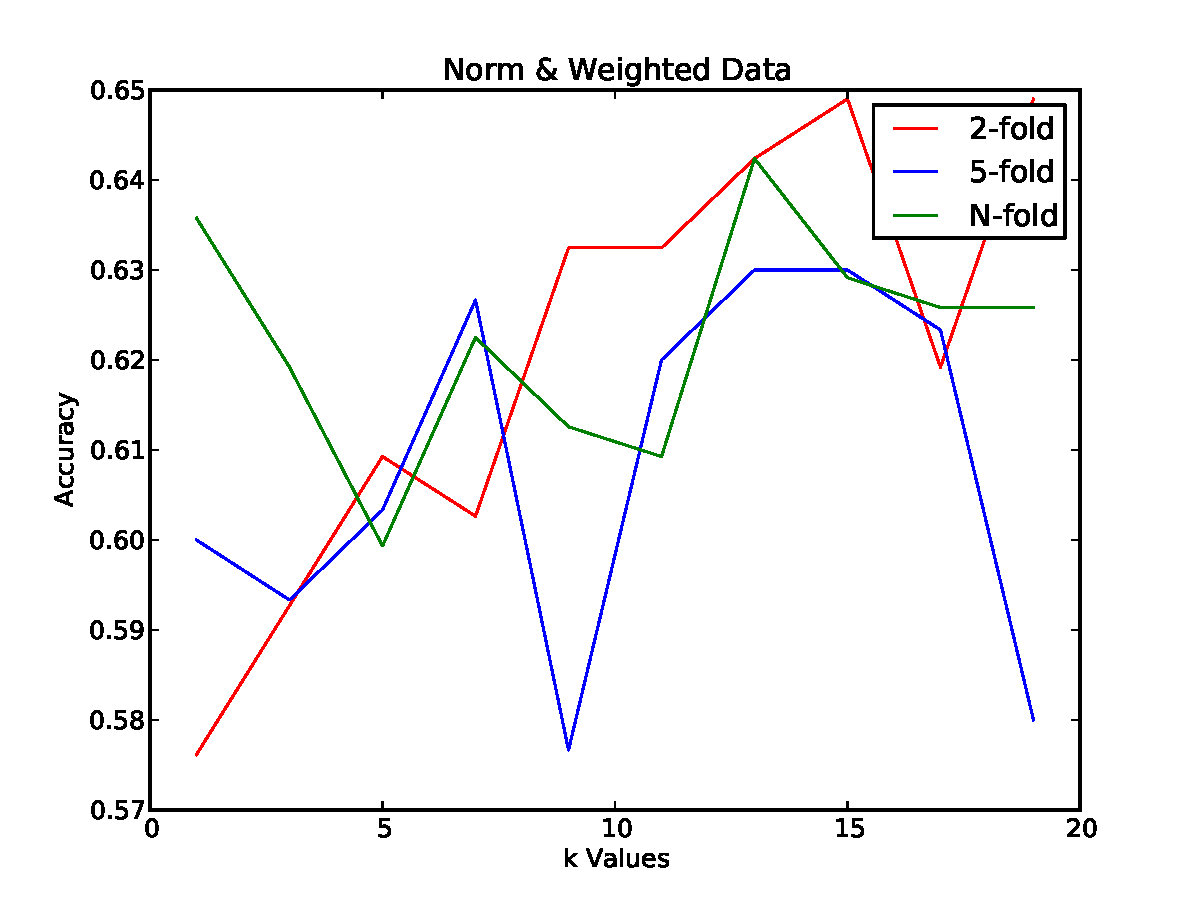
\includegraphics[width=2.8in]{images/alc_nw_100.pdf}
  \caption{100\% of the TD. At 100\% we see little stability due to the fact that the results are run only once and are therefore not an average of five iterations of a random subset.}
\end{figure}
\begin{figure}[h]
  \centering
  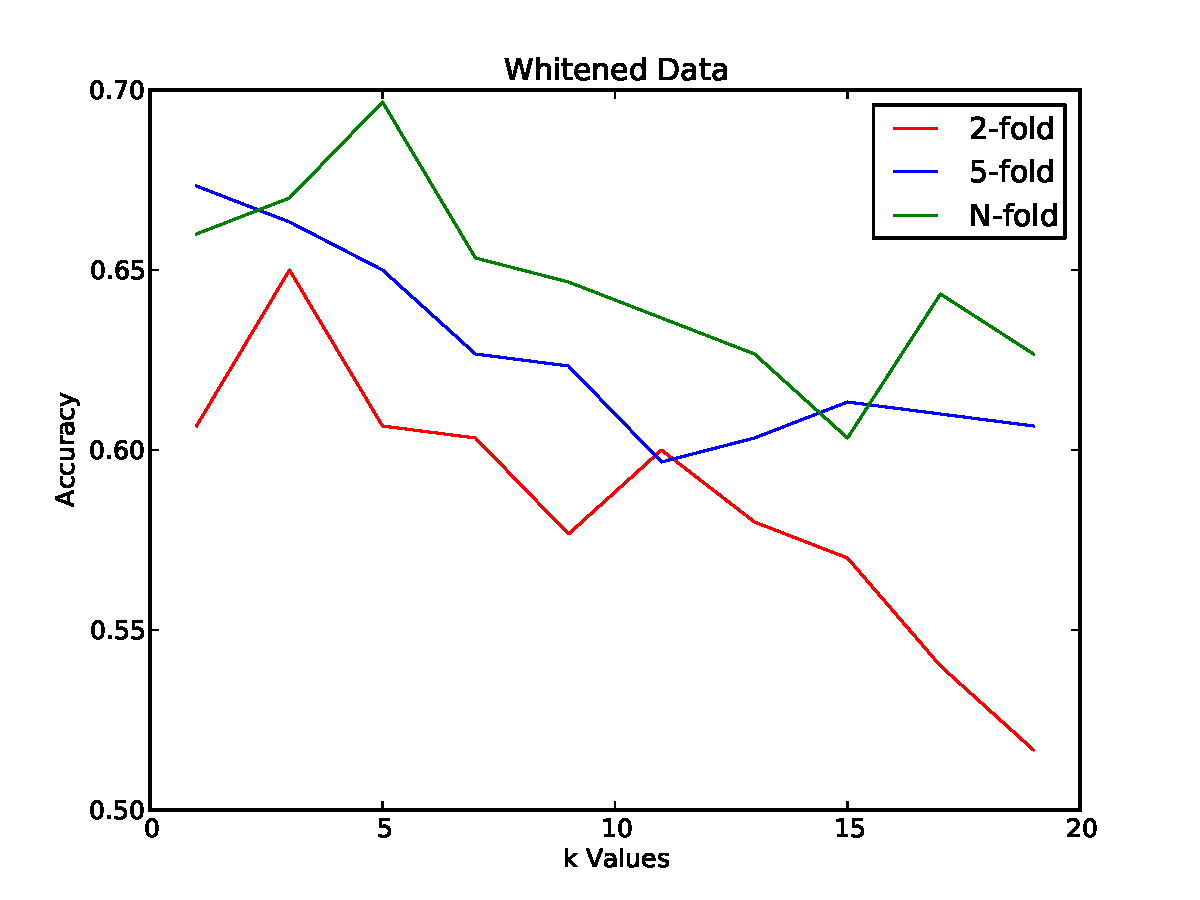
\includegraphics[width=2.8in]{images/alc_w_20.pdf}
  \caption{20\% of the TD. We see little to no correlation in the data here, which is expected given that you are randomly selecting 20 percent of the data, these training sets were unstable.}
\end{figure}
\begin{figure}[h]
  \centering
  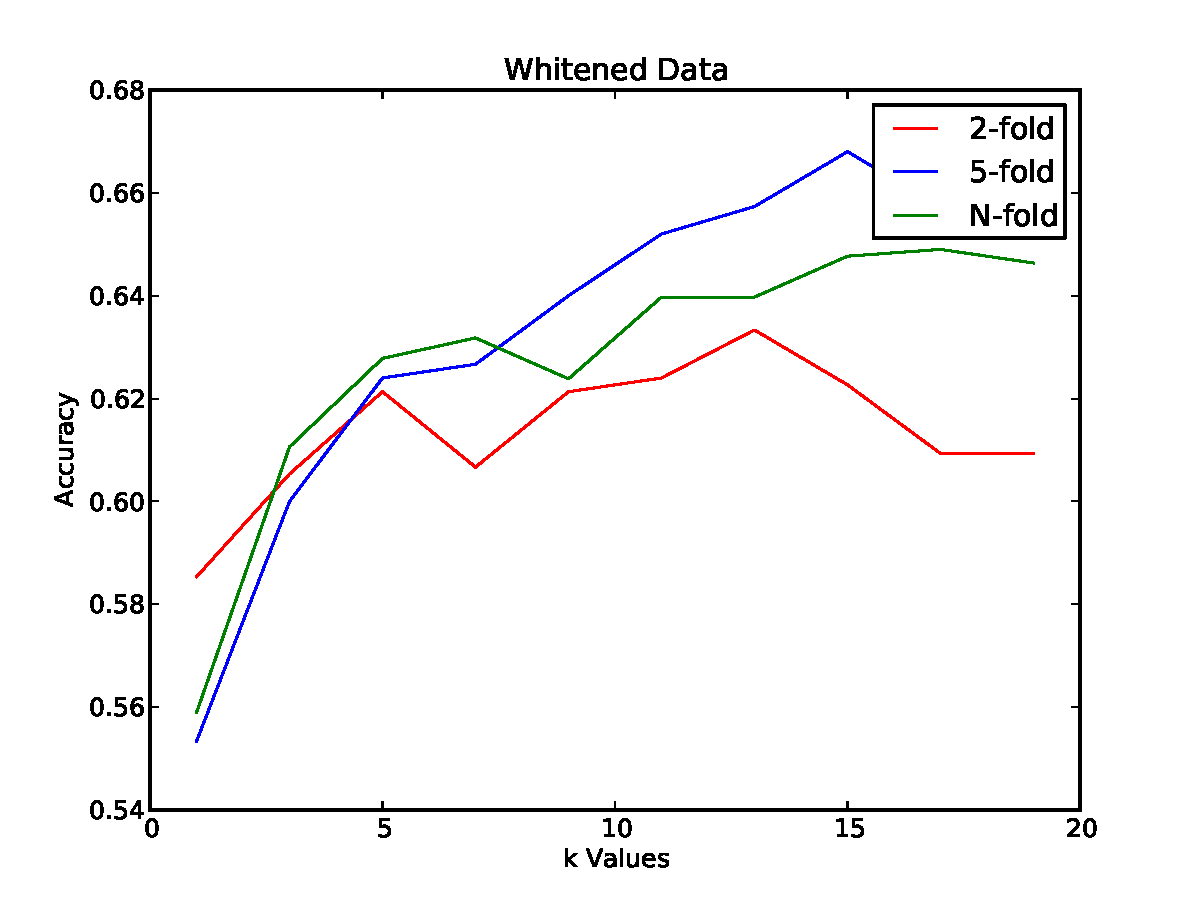
\includegraphics[width=2.8in]{images/alc_w_50.pdf}
  \caption{50\% of the TD. In this we see great stability and it is easier to view a trend based on the given k values.}
\end{figure}
\begin{figure}[h]
  \centering
  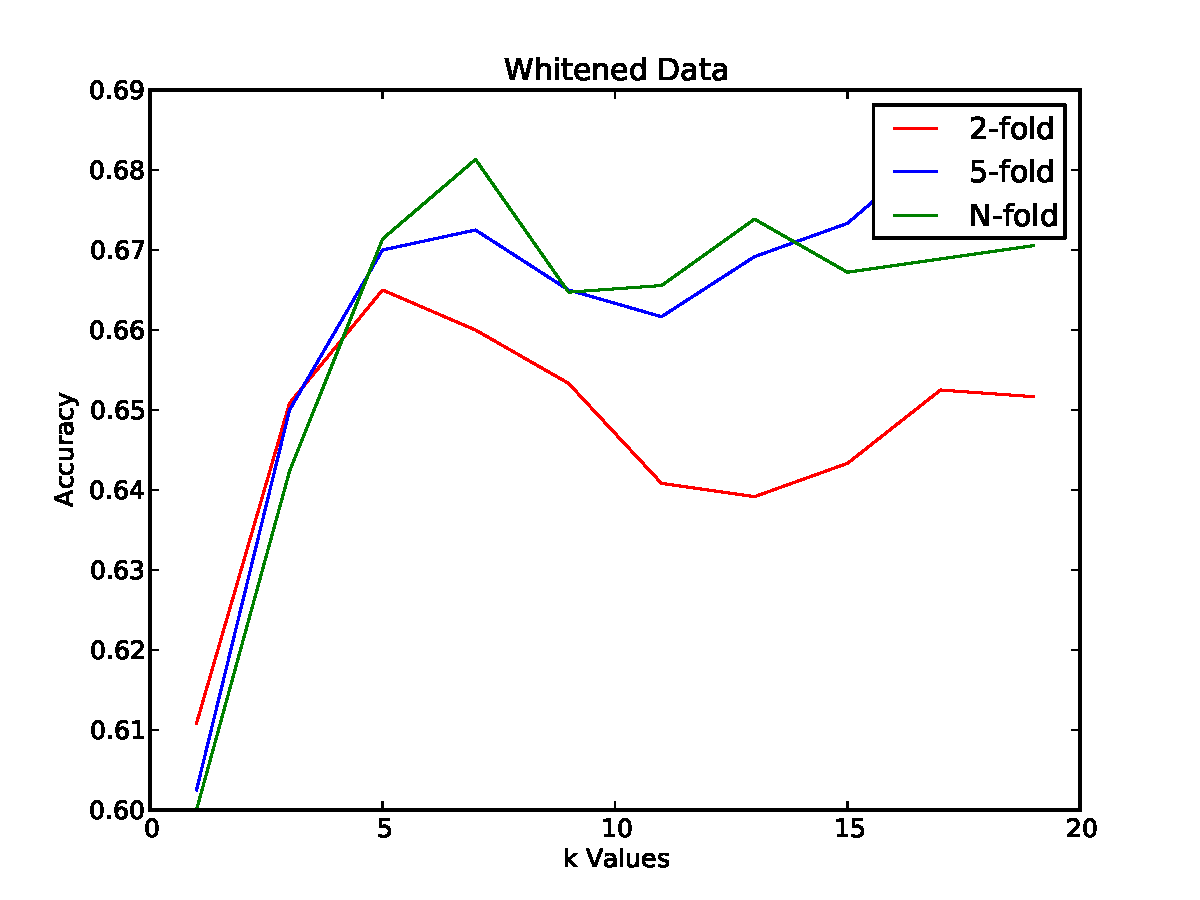
\includegraphics[width=2.8in]{images/alc_w_80.pdf}
  \caption{80\% of the TD. Here we see the greatest stability with 5-fold and N-fold CV converging to very similar classification results. 2-fold CV approaches a similar shape but at less accuracy.}
\end{figure}
\begin{figure}[t]
  \centering
  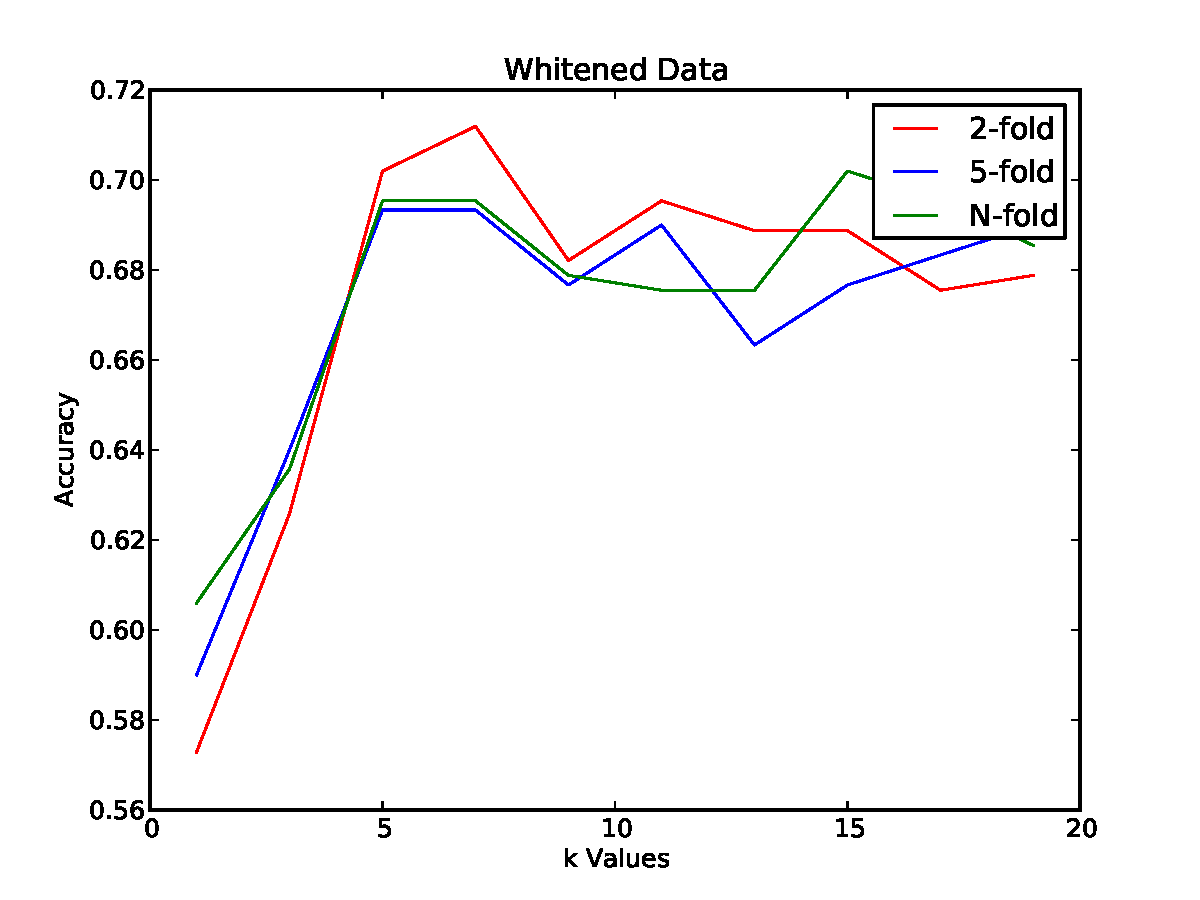
\includegraphics[width=2.8in]{images/alc_w_100.pdf}
  \caption{100\% of the TD. This becomes a lot more volatile because we are not running five iterations of a random subset (since this subset spans the entire set). Albeit the volatility, this achieves the highest accuracy with 7 nearest neighbors.}
\end{figure}
\end{document}
